%-----------------------------------------------------------------------------
% Based on 15 February 2005 sigplanconf-template.tex by Paul C. Anagnostopoulos
%-----------------------------------------------------------------------------

\documentclass[12pt]{article}

\usepackage{bibspacing}
\usepackage{times}
\usepackage{amsmath}
\usepackage{psfig}
\usepackage{url}

\usepackage{simplemargins}
\setleftmargin{1.25in}
\setrightmargin{1.25in}
\settopmargin{1in}
\setbottommargin{1in}

\makeatletter
\font\elvbf  = cmbx10 scaled 1100
\def\section{\@startsection {section}{1}{\z@}
   {12pt plus 2pt minus 2pt}{8pt plus 2pt minus 2pt} {\large\bf}}
\def\subsection{\@startsection {subsection}{2}{\z@}
   {10pt plus 2pt minus 2pt}{4pt plus 1pt minus 1pt} {\bf}}
\makeatother

\newcommand{\eightpoint}{\fontsize{8pt}{10pt}\selectfont}
\newcommand{\ninepoint}{\fontsize{9pt}{11pt}\selectfont}
\newcommand{\tenpoint}{\fontsize{10pt}{12pt}\selectfont}
\newcommand{\elevenpoint}{\fontsize{11pt}{13pt}\selectfont}
\newcommand{\thirteenpoint}{\fontsize{13pt}{14pt}\selectfont}
\newcommand{\fourteenpoint}{\fontsize{14pt}{16pt}\selectfont}

\begin{document}

%\conferenceinfo{POPL '06}{January 2007, Nice, France.} 
%\copyrightyear{2007}
%\copyrightdata{[to be supplied]}

%\titlebanner{banner above paper title}        % These are ignored unless
%\preprintfooter{short description of paper}   % 'preprint' option specified.

\title{\vspace{-40pt} \Large Direct Manipulation of LZ77-Compressed Data}
%\title{\vspace{-40pt} \Large Compressed-Domain Techniques for Lossless Formats}

%\title{\Large Compressed-Domain Techniques for Lempel-Ziv Formats}
%\title{\Large Compressed-Domain Transformation of Lossless Image and Video Encodings}

%\authorinfo{}

\author{\vspace{-24pt} ~ \\ \thirteenpoint William Thies, Steven Hall, and Saman Amarasinghe \\
        \thirteenpoint MIT Computer Science and Artificial Intelligence Laboratory \\ \vspace{-48pt}}

\date{}
%	    Massachusetts Institute of Technology}
%           {\{thies,saman\}@mit.edu}

\maketitle

\begin{abstract}
As DSP programming is becoming more complex, there is an increasing
need for high-level abstractions that can be efficiently compiled.
Toward this end, we present a set of aggressive optimizations that
target linear sections of a stream program.  Our input language is
StreamIt, which represents programs as a hierarchical graph of
autonomous filters.  A filter is linear if each of its outputs can be
represented as an affine combination of its inputs.  Linear filters
are common in DSP applications; examples include FIR filters,
expanders, compressors, FFTs and DCTs.

We present a linear extraction analysis that automatically detects
linear filters based on the C-like code in their {\tt work} function.
Once linear filters are identified, we show how neighboring nodes can
be collapsed into a single linear representation, thereby eliminating
many redundant computations.  Also, we describe a method for
automatically translating linear nodes into the frequency domain,
thereby yielding algorithmic savings for convolutional filters.

We have completed a fully-automatic implementation of the above
techniques as part of the StreamIt compiler, and we demonstrate
performance improvements that average 400\% over our benchmark
applications.




\end{abstract}

%% \category{CR-number}{subcategory}{third-level}
%%
%% \terms
%% term1, term2
%%
%% \keywords
%% keyword1, keyword2

\section{Introduction}

Applications that are structured around some notion of a ``stream''
are becoming increasingly important and widespread.  There is evidence
that streaming media applications are already consuming most of the
cycles on consumer machines \cite{Rix98}, and their use is continuing
to grow.  In the embedded domain, applications for hand-held
computers, cell phones, and DSP's are centered around a stream of
voice or video data.  The stream abstraction is also fundamental to
high-performance applications such as intelligent software routers,
cell phone base stations, and HDTV editing consoles.

Despite the prevalence of these applications, there is surprisingly
little language and compiler support for practical, large-scale stream
programming.  Of course, the notion of a stream as a programming
abstraction has been around for decades \cite{SICP}, and a number of
special-purpose stream languages have been designed (see
\cite{survey97} for a review).  Many of these languages and
representations are elegant and theoretically sound, but they often
lack features and are too inflexible to support straightforward
development of modern stream applications, or their implementations
are too inefficient to use in practice.  Consequently, most
programmers turn to general-purpose languages such as C or C++ to
implement stream programs.

There are two reasons that general-purpose languages are inadequate for
stream programming.  Firstly, they are a mismatch for the application
domain.  That is, they do not provide a natural or intuitive
representation of streams, thereby having a negative effect on
readability, robustness, and programmer productivity.  Moreover, because
the widespread parallelism and regular communication patterns of data
streams are left implicit in general-purpose languages, compilers are
not stream-conscious and do not perform stream-specific optimizations.
As a result, performance-critical loops are often hand-coded in a
low-level assembly language and must be re-implemented for each target
architecture.  This practice is labor-intensive, error-prone, and very
costly.

Secondly, general-purpose languages are a mismatch for the emerging
class of grid-based architectures \cite{smartmemories,rawshort,trips} that
are especially well-suited for stream processing.  Perhaps the primary
appeal of C is that it provides a ``common machine language'' for
von-Neumann architectures.  That is, it abstracts away the
idiosyncratic differences between machines, but encapsulates their
common properties: a single program counter, arithmetic operations,
and a monolithic memory.  However, for grid-based architectures, the
von-Neumann model no longer holds, as there are multiple instruction
streams and distributed memory banks.  Thus, C no longer serves as a
common machine language--in fact, it provides the wrong abstraction
for the underlying hardware, and architecture-specific directives are
often needed to obtain reasonable performance.  Again, this greatly
complicates the job of the programmer and hampers portability.

StreamIt is a language and compiler specifically designed for modern
stream programming.  The StreamIt language has two goals: first, to
provide high-level stream abstractions that improve programmer
productivity and program robustness within the streaming domain, and
second, to serve as a common machine language for grid-based
processors.  At the same time, the StreamIt compiler aims to perform
stream-specific optimizations to achieve the performance of an expert
programmer.

This paper motivates, describes, and justifies the high-level language
features of StreamIt, version 1.0.  The major limitation of StreamIt
1.0 is that all flow rates in the streams must be static; applications
such as compression that have dynamically varying flow rates will be
the subject of future work.  A large set of applications can be
implemented with static rates, and while dynamic rates will require a
different runtime model, it will still be essential to fully analyse
and optimize static sub-sections in order to obtain high performance.

The paper is organized as follows. In Section {\ref{sec:domain}}, we
characterize the domain of streaming programs that motivates the
design of StreamIt, and in Section~\ref{sec:overview} we describe the
language features in detail.  We present an in-depth example of a
software radio in Section~\ref{sec:example}, preliminary results in
Section~\ref{sec:results}, related work in Section~\ref{sec:related},
and conclusions in Section~\ref{sec:conc}.


% RULE APPEARANCE:
\newcommand{\x}{\hspace{1.3pt}} % arithmetic multiplication symbol
\newcommand{\concat}[0]{\bullet}               % list concatenation symbol
\newcommand{\name}[1]{~~\hfill\framebox{#1}}   % for labeling rules

% RULE SPACING:
\newcommand{\skiptop}[0]{\vspace{-13pt}\\}   % for single line on top
\newcommand{\skiptopa}[0]{\vspace{-1pt}\\}   % for first line of two-line top part
\newcommand{\skiptopb}[0]{\vspace{-3pt}\\}   % for second line of two-line top part
\newcommand{\skipbot}[0]{\vspace{-3pt}\\}    % for single line on botto

% HELPER FOR REPEATS:
\newcommand{\tup}[2]{\langle#1, #2\rangle}

% OUR LABEL FOR THE ``POS'' VARIABLE
\newcommand{\pos}[0]{\mbox{\it pos}}

% MY TAB STOP FOR THE PSEUDOCODE
\newcommand{\tab}[0]{\mbox{~~~~}}

%%%%%%%%%%%%%%%%%%%%%%%%%%%%%%%%%%%%%%%%%%%%%%%%%%%%%%%%%%%%%%%%%%%%%%%%%%

\enlargethispage{0.5pt}
\section{Program Representation}

Our transformation relies on the cyclo-static dataflow representation
for input programs and the LZ77 representation of compressed data.
These are described in the next two sections.

\subsection{Cyclo-Static Dataflow}

In the cyclo-static dataflow model, a program is represented by a set
of independent {\it actors} that communicate using FIFO data
channels~\cite{bilsen95-cyclostatic,LM87-i}.  Each actor has an
independent program counter and address space; all communication is
done using the data channels.  Actors have one or more atomic
execution steps that execute in a fixed pattern throughout the
lifetime of the program.  A key restriction of the cyclo-static
dataflow model is that, for each execution of a given actor, the
number of items produced and consumed on the data channels is known at
compile time.  This enables the compiler to perform static scheduling
of the actors and to guarantee deadlock freedom~\cite{bilsen95-cyclostatic,LM87-i}.

Cyclo-static dataflow is a natural fit for many multimedia and signal
processing kernels, as such programs often have a regular structure
with known communication patterns.  As a programmer, one can use a
high-level language such as StreamIt~\cite{streamitcc} to express a
cyclo-static dataflow program.  An example StreamIt program appears in
Figure~\ref{fig:streamit}.  It reads lines of an RGB image from a
file, shrinks the image by a factor of two, inverts the color of each
pixel, then writes the data to a file.  There are three kinds of
actors in StreamIt programs, and our analysis handles each one
separately:
\begin{itemize}

\item {\bf Filters} have a single input stream and a single output
  stream, and perform general-purpose computation.  Filters perform
  the same function on every execution (there is no cyclic pattern of
  computations).  For example, in the {\tt InvertColor} filter, the
  {\tt work} function specifies the atomic execution step; it declares
  that on each execution, it pops (inputs) 1 item from the input tape
  and pushes (outputs) 1 item to the output tape\footnote{Though
    StreamIt also allows filters to peek at the input stream (i.e., to
    perform a sliding window computation) and to maintain mutable
    state across executions, these features are uncommon in other
    stream languages and we do not support them in the current work.}.

\item {\bf Splitters} have a single input stream and multiple output
  streams, and perform pre-defined computations.  There are two types
  of splitters: {\it duplicate} splitters, which replicate their
  inputs to all of the target streams, and {\it roundrobin} splitters,
  which distribute the input items across the streams.  Roundrobin
  splitters are parameterized: roundrobin$(n_1, n_2)$ indicates that
  the first $n_1$ items are sent to the first output, and the next
  $n_2$ items are sent to the second output.  Splitters execute in a
  fine-grained, cyclo-static fashion: regardless of the parameters,
  each execution step passes only a single item from the input stream
  to an output stream.  In Figure~\ref{fig:streamit}, the splitter
  sends {\tt WIDTH} pixels in each direction, distributing the lines
  of the image across alternate streams.

\begin{figure}[t]
\psfig{figure=streamit-figure.eps,width=3.408in}
\caption{Example StreamIt program.
\protect\label{fig:streamit}}
\end{figure}

\item {\bf Joiners} have multiple input streams and a single output
  stream, and perform pre-defined computations.  The only type of
  joiner is roundrobin, which acts analogously to a roundrobin
  splitter.  In Figure~\ref{fig:streamit}, the joiner reads one pixel
  at a time from each input stream, serving to interleave the pixels
  from neighboring lines.  Once the pixels are interleaved, each group
  of 4 pixels is averaged together in order to decrease the picture
  width by two.

\end{itemize}

\subsection{LZ77 Compression}

LZ77 is a lossless, dictionary-based compression algorithm.  Named
after its creators Lempel and Ziv, who published the algorithm in
1977~\cite{lz77}, LZ77 is asymptotically optimal~\cite{wyner94optimal}
and forms the basis for many popular compression formats, including
ZIP, GZIP and PNG.  As described in Section~\ref{sec:formats}, LZ77
also serves as a generalization of simpler encodings such as Apple
Animation, Microsoft RLE, and Targa, allowing our transformations to
naturally extend to these formats.

\begin{figure}[t]
\begin{minipage}{1.6in}
\hspace{-5pt}\begin{tabular}{rcl}
stream&\hspace{-9pt}:=&\hspace{-9pt}value$^*$\\ ~ & ~
\end{tabular}
\end{minipage}
\begin{minipage}{1.8in}
\hspace{-5pt}\begin{tabular}{rcl}
stream&\hspace{-9pt}:=&\hspace{-9pt}(value~$|$~repeat)$^*$ ~ \\
repeat&\hspace{-9pt}:=&\hspace{-9pt}$\langle$distance, count$\rangle$
\end{tabular}
\end{minipage} 
~ \\
\begin{minipage}{1.6in}
(a) Uncompressed domain
\end{minipage}
(b) Compressed domain (LZ77)
\caption{Representation of data in the uncompressed and compressed
domains.  \protect\label{fig:domains}}
\end{figure}

The basic idea behind LZ77 is to utilize a sliding window of recently
encoded values as the dictionary for the compression algorithm.  In
the compressed data stream, there are two types of tokens: {\it
values} and {\it repeats} (see Figure~\ref{fig:domains}).  A value
indicates a token that should be copied directly to output of the
decoded stream.  A repeat contains two parts: a distance $d$ and a
count $c$; it indicates that the decoder should start at offset $d$
from the end of the decoded stream and copy a sequence of $c$ values
to the output.  The distances are bounded, which enables the decoder
to operate with a fixed buffer size.  It is important to note that the
count may exceed the distance, in which case some of the values
produced by a repeat operation are also copied by that operation.  For
example, a value A followed by a repeat $\tup{1}{3}$ results in an
output of ``A A A''.  An additional example of LZ77 decoding is given
in Figure~\ref{fig:lz77}.

\begin{figure}[t]
\begin{minipage}{0.21in}
\mbox{~}
\end{minipage}
\psfig{figure=lz77-figure.eps,width=2.6in}
\caption{Example of LZ77 decompression.
\protect\label{fig:lz77}}
\end{figure}

\section{Program Transformation}
Our program transformation inputs a cyclo-static dataflow program and
outputs an equivalent program in which all of the data channels use a
compressed representation.  One can think of this process as mapping
from the uncompressed domain to the compressed domain (see
Figure~\ref{fig:domains}).  Rather than modifying the code within the
actors, our transformation treats actors as black boxes and wraps them
in a new execution layer.  The transformation attempts to preserve as
much compression as possible without ever performing an explicit
re-compression step.  While there exist cases in which the output data
will not be as compressed as possible, under certain conditions the
output is guaranteed to be fully compressed (relative to the
compression of the input).

For the sake of presentation, we use an operational semantics to
express the execution under the uncompressed and compressed domains.
Though some of the transition rules require dynamic data rates and
thus fall outside the cyclo-static dataflow model, all of them have an
efficient implementation in StreamIt.  The rules use the notations
given in Figure~\ref{fig:notations}, and have the following form:

\hspace{-12pt}\begin{tabular}{l} ~ \vspace{-6pt} \\ 
\hspace{-3pt}$S \rightarrow T$ \hspace{-7pt}~\vspace{0.5pt} \\ \hline ~ \vspace{-7.5pt} \\
\hspace{-3pt}$S' \rightarrow T'$ \hspace{-7pt} \\ ~ \vspace{-6pt} \\
\end{tabular}

This rule reads: if the incoming stream has value $S$ and the outgoing
stream has value $T$, then after an execution step, the streams have
values $S'$ and $T'$, respectively.  As detailed in
Figure~\ref{fig:domains}, we represent streams as lists of tokens;
inputs to the stream are added to the front of the list, while outputs
from the stream are removed from the end of the list.

To describe the mapping into the compressed domain, we consider each
StreamIt construct in turn: filters, splitters, and joiners.

\subsection{Filters}

\newcommand{\tablesep}{\hspace{-3.5pt}}
\begin{figure}[t]
\hspace{-5pt}\begin{tabular}{llll}
\multicolumn{2}{l}{Variables} & \multicolumn{2}{l}{{\tablesep}Constants} \\ \rule[10pt]{1.9in}{0.3pt}\hspace{0.1in}\rule[10pt]{1.3in}{0.3pt}\hspace{-1.3in}\hspace{-2pt}\hspace{-1.97in}\hspace{-2pt}
$S$, $T$ & {\tablesep}Input, output streams & {\tablesep}$n_1$, $n_2$ & {\tablesep}Actor's pop rates \\
$V$ & {\tablesep}List of values (may be empty) & {\tablesep}$m$ & {\tablesep}Actor's push rate \\
$\tup{d}{c}$ & {\tablesep}Repeat distance \& count & {\tablesep}~ & ~ \vspace{6pt} \\
\multicolumn{2}{l}{Functions (list $\times$ list $\rightarrow$ list)}& ~ & ~ \\ \rule[10pt]{3.3in}{0.3pt}\hspace{-3.3in}
$\concat$ & {\tablesep}List concatenation & ~ & ~ \\
$F$ & \multicolumn{3}{l}{{\tablesep}Filter work function, outputs $m$-element list}
\end{tabular}
\caption{Notations used in the semantic rules.\protect\label{fig:notations}}
\end{figure}

\begin{figure}[t]
$S \concat V \rightarrow T~~~~|V|=n$\name{exec-uncompressed} \skiptopb
---------------------------- \skipbot
$S \rightarrow F(V) \concat T$
\caption{Semantics of \textsc{Exec(F)}: execution of filter F in the
uncompressed domain.  Notations are defined in Figure~\ref{fig:notations}.
\protect\label{fig:exec-rule}}
\end{figure}

\begin{figure}[t]
~~~~~~~~~\psfig{figure=actor-figure.eps,width=2.8in}

\mbox{~}(a) Uncompressed domain~~~~~~~~~~~~~~~~~(b) Compressed domain
\caption{Overall execution of a filter F in the uncompressed and compressed domains.
\protect\label{fig:actor-pic}}
\end{figure}

Filter execution in the uncompressed domain is described by the rule
in Figure~\ref{fig:exec-rule}.  The rule expresses the simple fact
that a filter inputs a list of $n$ values from the end of its input
stream; this list is denoted by $V$.  The filter pushes its results,
denoted by $F(V)$, onto the front of the output stream.

\begin{figure*}[t]
\vspace{-6pt}
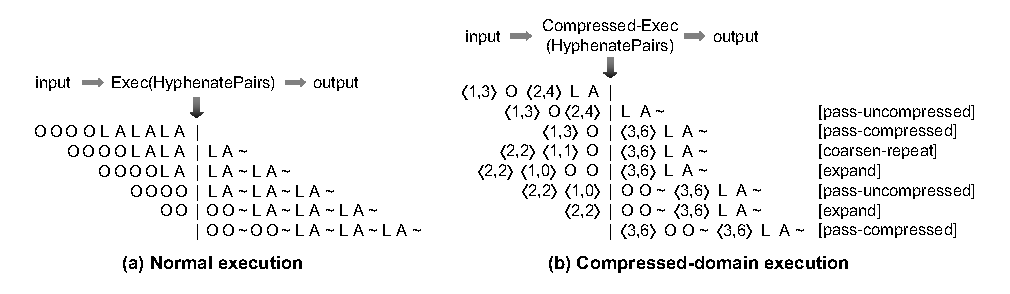
\psfig{file=compressed-filter-example.eps,width=\textwidth}
\vspace{6pt}
\caption{Example execution of a filter in the uncompressed and
  compressed domains.\protect\label{fig:filter-example}}
\end{figure*}

\begin{figure}[t]
$S \concat V \rightarrow T~~~~|V|=n$\name{exec-uncompressed} \skiptopb
---------------------------- \skipbot
$S \rightarrow F(V) \concat T$
~ \\ ~ \\
%\hfill\mbox{\it Same as above.}\name{exec-uncompressed}\vspace{6pt}\\
$S \concat \tup{d}{c} \rightarrow T~~~~d$\%$n=0~~~~c$\%$n=0$\name{exec-compressed} \skiptopb
------------------------------------------------ \skipbot
$S \rightarrow \tup{m{\x}d/n}{m{\x}c/n} \concat T$
\caption{Semantics of \textsc{Compressed-Exec(F)}: execution of filter
$F$ in the compressed domain.
%This filter also includes an {\tt exec-uncompressed} rule, which is
%identical to the one in Figure~\ref{fig:exec-rule}.
Notations are defined in Figure~\ref{fig:notations}.
\protect\label{fig:compressed-exec-rule}}
\end{figure}

Filter execution in the compressed domain requires a two-stage
transformation (see Figure~\ref{fig:actor-pic} for an overview, and
Figure~\ref{fig:filter-example} for a detailed example).  First, the
input stream is aligned to a granularity $n$ that matches the input
rate of the filter.  This alignment guarantees that every token in the
stream is either a sequence of $n$ values, or a repeat in which both
the distance and the count are multiples of $n$.  The alignment stage
(described in detail later) is a no-op for filters that pop only one
item ($n=1$).

After the alignment stage comes the execution of the compressed
filter, which appears in Figure~\ref{fig:compressed-exec-rule}.  The
{\tt exec-uncompressed} rule
%(not shown in Figure~\ref{fig:compressed-exec-rule}) 
deals with values on the input stream, and is identical to that in the
uncompressed execution.  The {\tt exec-compressed} rule deals with
repeats on the input stream and encapsulates the key idea of the
paper.  Because the inputs are repeating at the correct granularity,
the repeat can be copied directly to the output of the filter without
performing any new computation.  The only change needed is to adjust
the repeat distance and count to match the filter's output rate.

\subsubsection{Stream Alignment}

The alignment phase is needed for filters that pop more than one item
from the input stream.  Its goal is to align the execution boundaries
of the filter with the repeat boundaries of the compressed data; this
alignment is required for the compressed execution.  Following
alignment, each execution of a filter will input either $n$
consecutive values, or a repeat token with a distance and count that
are evenly divisible by $n$ (where $n$ represents the pop rate of the
filter).

The alignment stage sometimes needs to partially decompress the data
in the stream.  Due to the sliding-window dictionary in LZ77, in
general it is difficult to decode only a few items without
decompressing others.  Thus, our formulation assumes that a fully
decompressed version of the stream is available; the transition rules
access the decompressed data using the \mbox{\it decode} function,
which returns the sequence of values represented by a repeat token at
its current position in the stream.  However, in practice, this
decompression can be avoided whenever the repeat distance is the same
as the window size, as this simply causes a value in the window to be
overwritten by itself.  This case is very common in several practical
compression formats; for example, in Apple Animation, the vast
majority of repeats reference the same pixel in the previous frame
(which is also the window size), and thus most decompression is
avoided.  In run-length encoding, the repeat distance and the window
size are always equal to one, so no decompression is needed.  While
general LZ77 does require a decompressed window to be maintained, our
technique still offers significant benefits by computing on a smaller
volume of data and avoiding the cost of re-compression.  For general
algorithms such as gzip, compression can be up to 10x slower than
decompression~\cite{ziviani00compression}.

The semantics of stream alignment are given in
Figure~\ref{fig:stream-align}.  If the end of the input stream
contains $n$ values, then alignment is satisfied and the values are
moved to the output stream (rule {\tt pass-uncompressed}).  Likewise,
if the input contains a repeat in which the distance is a multiple of
$n$ and the count is at least $n$, then a number of aligned repeats
are peeled from the input and moved to the output (rule {\tt
  pass-compressed}).  If the count is not a multiple of $n$, then part
of the repeat is leftover and remains on the input stream.

There are some cases in which a repeat cannot be moved to the output
stream, in which case the data needs to be partially decompressed
(rule {\tt expand}).  This occurs if the repeat has a count less than
$n$, if it occurs in the middle of an aligned stretch of $n$ values,
or if its distance is not a multiple of $n$ (this last condition can
sometimes be remedied by another rule, see below).  The {\tt expand}
rule decodes only one value from an unaligned repeat token, thereby
decreasing its count by one; the rest of the repeat may become aligned
later.  If the count of a repeat reaches zero, it is eliminated by the
{\tt prune} rule.

\begin{figure}[t]
$S \concat V \rightarrow T~~~|V|=n$\name{pass-uncompressed}\skiptopb
---------------------------\skipbot
$S \rightarrow V \concat T$
~ \\ ~ \\
$S \concat \tup{d}{c} \rightarrow T~~~d$\%$n=0~~~c \ge n$\name{pass-compressed}\skiptopb
------------------------------------------\skipbot
$S \concat \tup{d}{c$\%$n} \rightarrow \tup{d}{c-c$\%$n} \concat T$
~ \\ ~ \\
$S \concat \tup{d}{c} \concat V \rightarrow T$\name{expand}\\
$c<n~\vee~1 \le |V|<n~\vee~(d$\%$n>0~\wedge~\neg(d < \mbox{LCM}(d,n) < c))$\skiptopb
--------------------------------------------------------------------------------\skipbot
$S \concat \tup{d}{c-1} \concat \mbox{\it decode}(\tup{d}{1}) \concat V \rightarrow T$
~ \\ ~ \\
$S \concat \tup{d}{0} \concat V \rightarrow T$\name{prune}\skiptopb
------------------------\skipbot
$S \concat V \rightarrow T$
~ \\ ~ \\
let~$L=\mbox{LCM}(d,n)$\name{coarsen-repeat}\\
$S \concat \tup{d}{c} \concat V \rightarrow T~~~~d$\%$n > 0~~~~d < L < c$\vspace{-3pt}\skiptopa
-------------------------------------------------------\skipbot
$S \concat \tup{L}{c-(L-d)} \concat \tup{d}{L-d} \concat V \rightarrow T$
\caption{Semantics of \textsc{Align}($n$): aligning data
to a granularity of $n$.  The \mbox{\it decode} function uncompresses
a repeat token into a list of values; other notations are given in
Figure~\ref{fig:notations}. \protect\label{fig:stream-align}}
\end{figure}

The final rule, {\tt coarsen-repeat}, preserves a specific kind of
compression in the input stream.  Consider that a filter pops two
items at a time, but encounters a long repeat with distance three and
count 100.  That is, the input stream contains a regular pattern of
values with periodicity three.  Though consecutive executions of the
filter are aligned at different offsets in this pattern, every third
filter execution (spanning six values) falls at the same alignment.
In general, a repeat with distance $d$ can be exploited by a filter
with pop rate $n$ by expanding the distance to $\mbox{LCM}(d, n)$.  In
order to perform this expansion, the count must be greater than the
distance, as otherwise the repeat references old data that may have no
periodicity.  Also, the stream needs to be padded with $\mbox{LCM}-d$
values before the coarsened repeat can begin; this padding takes the
form of a shorter repeat using the original distance.

%% NOTE: the second point made in this section is not quite true,
%% since you still need to decompress RLE units that are a frame away
%% in Apple Animation.  Also first point seems redundant with align
%% being no-op for pop=1, so not including this.
%%
%% \subsubsection{Optimizations}
%% \label{sec:opt}
%%
%% As the transformation to the compressed domain is formulated in
%% fully general terms, the process can be streamlined considerably for
%% common classes of inputs:
%% \begin{itemize}
%% \item If a filter has a pop rate of one ($n=1$) on a given stream then
%%   no alignment stage is needed.
%% \item If the repeat distance is equal to the LZ77 window size, then no
%%   decompression is needed because it would simply overwrite the same
%%   values in the buffer.  This property holds for inter-frame repeats
%%   in the Apple Animation format (see Section~\ref{sec:formats}).
%% \end{itemize}
%% A consequence of the first bullet is that filters with a pop rate of
%% one (such as the InvertColor filter in Figure~\ref{fig:streamit}) avoid
%% performing any decompression, as there is no alignment stage.  This
%% guarantees that the output of the filter will be the same size as the
%% compressed input.

%% \subsection{Extensions}
%% \label{sec:extensions}

%% The transformation can be extended to support a broader class of
%% filters.  Some straightforward extensions are as follows:
%% \begin{itemize}

%% \item {\it Filters with state.}  If a filter retains mutable state from
%% one execution to the next, a repeat token can be copied across the
%% filter if the current state values are the same as they were at the
%% beginning of the repeated segment.  One could maintain a lookup table
%% that tracks the state values for the sake of this comparison.  Also,
%% state updates that have a closed form can be applied in the compressed
%% domain even if the current state has never been seen before; for
%% example, if a histogram filter runs for $n$ iterations on a blue
%% pixel, it will increment the blue count by $n$ regardless of the
%% initial value.

%% \item {\it Dynamic input and output rates.}  The current formulation
%% relies on a filter's fixed I/O rates to calculate repeat distances and
%% counts for the output tape from the repeat tokens on the input tapes.
%% However, in the presence of unpredictable I/O rates (e.g., edge
%% detection), a lookup table could be used to track the actual I/O rates
%% on each execution.  In the event of a repeat, the recorded I/O rates
%% from the previous execution could be used to calculate the repeat
%% parameters on the output tape.

%% \item {\it Sliding window computations.}  We currently assume that an
%% filter consumes all of the items it inspects on a given execution step.
%% However, some filters (e.g., a Gaussian blur filter) inspect a window
%% of values in addition to the one that is consumed.  Such {\it peeking}
%% filters can be supported by adjusting the translation of repeat
%% tokens, shortening the output count to match the period that the
%% entire window was within the repeated range.

%% \end{itemize}

\subsection{Splitters}

It is necessary to consider splitters and joiners separately from
general-purpose actors because of their pass-through semantics: the
inputs are distributed to the outputs without performing any
computation.  Our translation to the compressed domain leverages this
fact to preserve considerably more compression than would be possible
if splitters and joiners were viewed as opaque computational nodes
with multiple inputs and multiple outputs.  Consequently, splitters
and joiners should be employed by the programmer not only as a natural
expression of parallelism, but as a powerful way of exposing the data
reordering to the compiler.

As mentioned previously, splitters and joiners adopt a fine-grained
cyclo-static execution model, in which each execution step transfers
only one item from an input tape to an output tape.  That is, a
roundrobin$(k_1, k_2)$ splitter or joiner has $k_1 + k_2$ distinct
execution steps.  We refer to every group of $k_1 + k_2$ steps as an
{\it execution cycle}.

Duplicate splitters are trivial to transform to the compressed domain,
as all input tokens (both values and repeats) are copied directly to
the output streams.  For roundrobin splitters, the central concern is
that a repeat token can only be transferred to a given output tape if
the items referenced are also on that tape.  If the items referenced
by the repeat token were distributed to another tape, then the repeat
must be decompressed.

\begin{figure}[t]
\vspace{-1pt} % makes a page break difference, amazing
~~~~~~~~~\psfig{figure=sj-figure.eps,width=2.8in}

\mbox{~~~~~~~~~~}(a) Notation for splitters~~~~~~~~~~~~~~(b) Notation for joiners
\caption{Notations used in the semantics for splitters and joiners.
  In addition, the variable $\pos$ indicates how many items have been
  written to (in the case of splitters) or read from (in the case of
  joiners) the active tape during the current execution cycle.
  \protect\label{fig:sj-pic}}
\end{figure}

The rest of this section focuses on roundrobin splitters.  To simplify
the presentation, we consider a splitter with only two output streams.
This captures all of the fundamental ideas; extension to additional
streams is straightforward.  Rewrite rules now take the following
form:

\hspace{-12pt}\begin{tabular}{l} ~ \vspace{-6pt} \\ 
\hspace{-3pt}$S \rightarrow T_1; T_2$ \hspace{-7pt}~\vspace{0.5pt} \\ \hline ~ \vspace{-7.5pt} \\
\hspace{-3pt}$S' \rightarrow T_1'; T_2'$ \hspace{-7pt} \\ ~ \vspace{-6pt} \\
\end{tabular}

\noindent where $T_1$ and $T_2$ represent the output streams of the
splitter (see Figure~\ref{fig:sj-pic}).  In addition, we make two
further simplifications:
\begin{itemize}

\item The rules assume that the next execution step of the splitter
  will write to $T_1$.  The subscripts should be interpreted without
  loss of generality.

\item We use $\pos$ to denote the number of items (in terms of the
  uncompressed domain) that have already been written to the current
  output stream ($T_1$) in the current execution cycle.  For brevity,
  the rules do not maintain the value of $\pos$, though it is
  straightforward to do so.

\end{itemize}

The semantics for splitter execution in the uncompressed domain appear
in Figure~\ref{fig:uncompressed-splitter}.  The {\tt
  pass-uncompressed} rule simply passes a single value from the input
tape to the current output tape, $T_1$.  Note that the current
position $\pos$ is implicitly incremented; once $\pos$ reaches $m_1$,
it is reset to zero and the output tapes are switched (tape $T_2$ will
be named $T_1$ on the next execution).

The compressed-domain semantics for splitters are given in
Figure~\ref{fig:compressed-splitter}, and a detailed example appears
in Figure~\ref{fig:sj-example}.  As mentioned previously, a repeat
token can be transferred to an output tape so long as the items
referenced also appear on that tape.  However, the repeat may need to
be fragmented (into several repeats of a lesser count), depending on
the repeat distance.  There are two cases to consider.

\begin{figure}[t]
$S \concat V \rightarrow T_1; T_2~~~~|V|=1$\name{pass-uncompressed}\skiptopb
---------------------------------\skipbot
$S \rightarrow V \concat T_1; T_2$
\caption{Semantics of \textsc{Splitter}: execution of a roundrobin
  splitter in the uncompressed domain.
 \protect\label{fig:uncompressed-splitter}}
\end{figure}

\begin{figure}[t]
$S \concat V \rightarrow T_1; T_2~~~~|V|=1$\name{pass-uncompressed}\skiptopb
---------------------------------\skipbot
$S \rightarrow V \concat T_1; T_2$
~ \\ ~ \\
let~$\mbox{offset} = d$\%$(m_1+m_2)$\name{pass-compressed-long}\skiptopb
let~$(L_1, L_2) = \mbox{run\_splitter}(c)$\vspace{2pt}\\
$S \concat \tup{d}{c} \rightarrow T_1; T_2~~~~\mbox{offset} = 0$\vspace{-3pt}\skiptopa
--------------------------------------------\skipbot
$S \rightarrow \tup{d{\x}m_1/(m_1+m_2)}{L_1} \concat T_1;$\\
\mbox{~~~~~~~~~}\hspace{0.29pt}$\tup{d{\x}m_2/(m_1+m_2)}{L_2} \concat T_2$
~ \\ ~ \\
let~$\mbox{offset} = d$\%$(m_1+m_2)$\name{pass-compressed-short}\skiptopb
let~$\mbox{offset'} = \mbox{\bf if~} \mbox{offset} \leq \pos \mbox{\bf ~then~} \mbox{offset}$\\
\mbox{~}\hspace{42.3pt}$\mbox{\bf ~else~} \mbox{offset} - m_2$\\
let~$\mbox{actual\_repeat} = \mbox{min}(c, \mbox{split\_potential}(d))$\\
$S \concat \tup{d}{c} \rightarrow T_1; T_2~~~~\mbox{offset} > 0~~~~\mbox{split\_potential}(d) > 0$\skiptopb
-------------------------------------------------------------------------\skipbot
$S \concat \tup{d}{c - \mbox{actual\_repeat}} \rightarrow$\\
$\tup{m_1*\mbox{floor}(d / (m_1 + m_2)) + \mbox{offset'}}{\mbox{actual\_repeat}} \concat T_1; T_2$
~ \\ ~ \\
let~$\mbox{offset} = d$\%$(m_1+m_2)$\name{expand}\skiptopb
$S \concat \tup{d}{c} \rightarrow T_1; T_2~~\hspace{1pt}\mbox{offset} > 0~~\hspace{1pt}\mbox{split\_potential}(d) = 0$\skiptopb
-------------------------------------------------------------------\skipbot
$S \concat \tup{d}{c-1} \concat \mbox{\it decode}(\tup{d}{1}) \rightarrow T_1; T_2$
~ \\ ~ \\
$S \concat \tup{d}{0} \rightarrow T_1; T_2$\name{prune}\skiptopb
------------------------\skipbot
$S \rightarrow T_1; T_2$
\caption{Semantics of \textsc{Compressed-Splitter}:  execution of a roundrobin
splitter in the compressed domain.
\protect\label{fig:compressed-splitter}}
\end{figure}

% improve this explanation
The first case, expressed by the {\tt pass-compressed-long} rule in
Figure~\ref{fig:compressed-splitter}, distributes an entire repeat
token to both output tapes without any fragmentation.  This is only
possible when the repeat can be cleanly separated into two independent
sequences, one offset by $m_1$ and the next offset by $m_2$.  In other
words, the repeat distance must be a multiple of $m_1+m_2$.  In this
case, the repeat token is moved to the output streams.  The repeat
distance is scaled down to match the weight of each stream, and the
count is divided according to the current position of the splitter (a
simple but tedious calculation implemented by {\tt run\_splitter} in
Figure~\ref{fig:helper-splitter}).

\begin{figure*}[t]
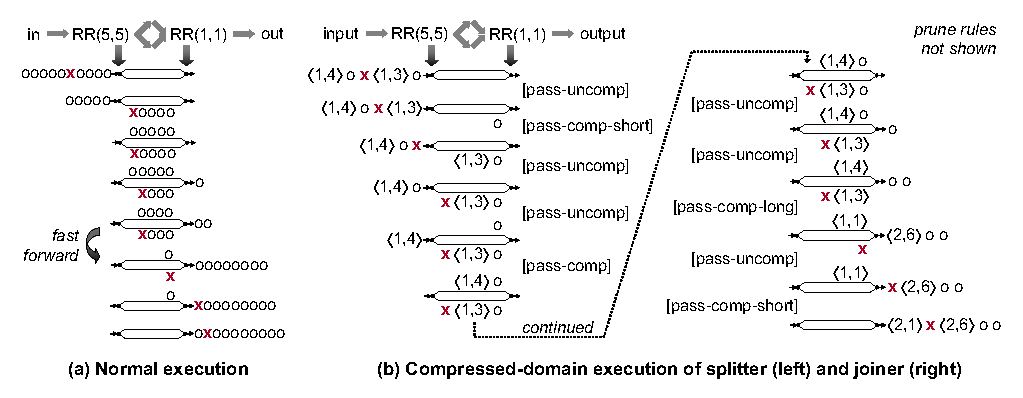
\psfig{file=compressed-splitjoin-example.eps,width=\textwidth}
\vspace{6pt}
\caption{Example execution of splitters and joiners in the compressed
  domain.  As illustrated by the input/output pairs in (a), the
  example performs a transpose of a 2x5 matrix.  When the matrix is
  linearized (as in (b) and (c)), the input stream traverses the
  elements row-wise while the output stream traverses column-wise.
  Due to redundancy in the matrix, this reordering can be done largely
  in the compressed domain.  \protect\label{fig:sj-example}}
\end{figure*}

\begin{figure}[t]
\begin{minipage}{0.1in}
\vspace{-1.75pt}
{\it // // // // //}
\end{minipage}
\begin{minipage}{3.23in}
{\it Given that $c$ items are available on input stream of a splitter,
  returns the number of items that can be written to each output stream
  before the input is exhausted.
  Assumes that the splitter is currently writing to the first output
  stream, to which \mbox{pos} items have previously been written in
  the current execution cycle.}
\end{minipage}
\mbox{\bf run\_splitter}$(c, \pos )$~returns~(int,~int)~\{\\
\tab{\it // the number of complete splitter cycles, and the leftover}\\
\tab$\mbox{total\_cycles} = \mbox{floor}(c/(m_1 + m_2))$\\
\tab$\mbox{total\_leftover} = c$\%$(m_1 + m_2)$\\
~ \vspace{-6pt}\\ 
\tab{\it // the last partial cycle may end in three regions:}\\
\tab$\mbox{\bf if~} \mbox{total\_leftover} \leq m_1 - \pos$~\{\\
\tab\tab{\it // 1. in writing to the first output stream}\\
\tab\tab$L_1 = \mbox{total\_leftover}$\\
\tab\tab$L_2 = 0$\\
\tab$\} \mbox{\bf~else if~} \mbox{total\_leftover} \leq m_1-\pos + m_2~\{$\\
\tab\tab{\it // 2. in subsequent writing to the second output stream}\\
\tab\tab$L_1 = m_1-\pos$\\
\tab\tab$L_2 = \mbox{total\_leftover} - m_1-\pos$\\
\tab\} \mbox{\bf else} \{\\
\tab\tab{\it // 3. in wrap-around writing to the first output stream}\\
\tab\tab$L_1 = \mbox{total\_leftover} - m_2$\\
\tab\tab$L_2 = m_2$\\
\tab\}\\
~ \vspace{-6pt}\\
\tab$\mbox{\bf return~}(m_1*\mbox{total\_cycles} + L_1, m_2*\mbox{total\_cycles} + L_2)$
\}\\
~ \\
\begin{minipage}{0.1in}
\vspace{-1.75pt}
{\it // // // // //}
\end{minipage}
\begin{minipage}{3.23in}
{\it Given a repeat token with distance $d$ that is input to a
  splitter, returns the maximum count of a repeat token that could
  safely be emitted to the current output stream of the splitter.
  Assumes that only a single repeat token can be emitted (i.e., the
  {\tt pass-compressed-long} rule does not apply).}
\end{minipage}
\mbox{\bf split\_potential}$(d)$~returns~int~\{\\
\tab$\mbox{offset} = d$\%$(m_1 + m_2)$\\
\tab$\mbox{{\bf if~}} \mbox{offset} \leq \pos ~\{$\\
\tab\tab{\it // repeat for remainder of this execution cycle}\\
\tab\tab$\mbox{\bf return~} m_1 - \pos$\\
\tab$\} \mbox{\bf ~else if~} \mbox{offset} > m_2 + \pos ~\{$\\
\tab\tab{\it // repeat until referenced data goes out of range}\\
\tab\tab$\mbox{\bf return~} \mbox{offset} - (m_2 + \pos)$\\
\tab$\} \mbox{\bf ~else} ~\{$\\
\tab\tab{\it // referenced data is on the other output stream}\\
\tab\tab$\mbox{\bf return~} 0$\\
\tab$\}$\\
\}
\caption{Helper functions for \textsc{Compressed-Splitter}.
\protect\label{fig:helper-splitter}}
\end{figure}

The second case, handled by the {\tt pass-compressed-short} rule, is
when the repeat distance is mis-aligned with the splitter's execution
cycle, and thus the repeat (if it is long enough) eventually
references items that are distributed to a different output tape.
Nonetheless, part of the repeat may be eligible to pass through, so
long as the items referenced refer to the current output tape.  This
judgment is performed by {\tt split\_potential}
(Figure~\ref{fig:helper-splitter}) by comparing the repeat distance to
the current position in the output stream.  If one or more of the
repeated values are in range, the valid segment of the repeat (of
length {\tt actual\_repeat}) is moved to the output tape.  As before,
the repeat distance needs to be scaled according to the weights of the
splitter, and an extra offset is needed if the repeat distance wraps
around to reference the end of a previous cycle.

If neither of the above transfers apply, then the input stream needs
to be partially decompressed (according to the {\tt expand} rule)
because the current repeat token references items that will be sent to
the wrong output tape.  The {\tt prune} rule is also needed to clear
empty repeats generated by {\tt expand}.

Though we omit the details, it is also desirable to employ an analog
of the {\tt coarsen-repeat} rule (Figure~\ref{fig:stream-align}) to
preserve even more compression across a splitter.  The intuition is
that, by increasing certain repeat distances, the splitter's output
tapes can become more independent (referencing themselves rather than
each other).  This enables a compressed rule to fire in place of an
expansion step.

\subsection{Joiners}

Analogously to splitters, there are two ways to pass repeat tokens
through a joiner.  If the input streams contain compatible repeat
tokens, then they can be combined into a long repeat that spans
multiple execution cycles; otherwise, a shorter repeat is extracted
from only one of the streams.  Both of these cases are illustrated by
example in Figure~\ref{fig:sj-example}.  Unlike splitters, there is
never a need to decompress repeat tokens into values before passing
through a joiner.  Though the repeat length may shrink to one, it will
remain a reference to a previous item rather than becoming a value
itself.

In the uncompressed domain, joiners have the semantics given in
Figure~\ref{fig:uncompressed-joiner}.  The {\tt pass-uncompressed}
rule passes a single value from the current input tape ($S_1$) to the
output tape.  Analogously to splitters, the variable $\pos$ represents
the number of items that have been read from the current input tape
and is implicitly updated.  Once $\pos$ reaches $n_1$, it is reset to
zero and the input tapes are switched (tape $S_2$ will be named $S_1$
on the next execution).

The first and most powerful way to execute joiners in the compressed
domain is to combine repeat tokens from both input streams
%
\clearpage\noindent\clearpage\noindent % WTF - with just 1 it gets really weird!
%
(rule {\tt pass-compressed-long} in
Figure~\ref{fig:compressed-joiner}).  For this to be possible, both
repeat distances must be the same multiple of their respective joiner
weight ($n_1$ or $n_2$); the combined token has a repeat distance that
is a multiple of $n_1 + n_2$.  The {\tt run\_joiner} routine
(Figure~\ref{fig:helper-joiner}) calculates the maximum repeat length
depending on the current position of the joiner and the repeat lengths
of the inputs.

\begin{figure}[t]
$S_1 \concat V; S_2 \rightarrow T~~~~|V|=1$\name{pass-uncompressed}\skiptopb
---------------------------------\skipbot
$S_1; S_2 \rightarrow V \concat T$
\caption{Semantics of \textsc{Joiner}: execution of a roundrobin
  joiner in the uncompressed domain.
\protect\label{fig:uncompressed-joiner}}
\end{figure}

\begin{figure}
$S_1 \concat V; S_2 \rightarrow T~~~~|V|=1$\name{pass-uncompressed}\skiptopb
---------------------------------\skipbot
$S_1; S_2 \rightarrow V \concat T$
~ \\ ~ \\
let~$(L_1, L_2) = \mbox{run\_joiner}(c_1, c_2, pos)$\name{pass-compressed-long}\skiptopb
$S_1 \concat \tup{d_1}{c_1};$\\
$S_2 \concat \tup{d_2}{c_2} \rightarrow T~~~~d_1$\%$n_1=0~~~~d_2$\%$n_2=0~~~~d_1/n_1=d_2/n_2$\vspace{-3pt}\skiptopa
--------------------------------------------------------------------------------\skipbot
$S_1 \concat \tup{d_1}{c_1-L_1};$\\
$S_2 \concat \tup{d_2}{c_2-L_2} \rightarrow \tup{d_1(n_1+n_2)/n_1}{L_1+L_2} \concat T$
~ \\ ~ \\
let~$\mbox{offset'} = \mbox{\bf ~if~} d$\%$n_1 \leq \pos \mbox{\bf ~then~} \pos$\name{\hspace{-0.5pt}pass-compressed-short\hspace{1.5pt}(a)\hspace{-0.5pt}}\skiptopb
$\mbox{~~~~}\hspace{37.7pt}\mbox{\bf ~else~} d$\%$n_1 + n_2$\\
let~$L=\mbox{min}(c,\mbox{join\_potential}(d))$\\
$S_1 \concat \tup{d}{c}; S_2 \concat V \rightarrow T$\vspace{-3pt}\skiptopa
--------------------------------------------------\skipbot
$S_1 \concat \tup{d}{c-L}; S_2 \concat V \rightarrow$\\
$\tup{(n_1 + n_2){\x}\mbox{floor}(d/n_1) + \mbox{offset'}}{L} \concat T$
~ \\ ~ \\
let~$\mbox{offset'} = \mbox{\bf ~if~} d$\%$n_1 \leq \pos \mbox{\bf ~then~} \pos$\name{\hspace{-0.7pt}pass-compressed-short\hspace{1.5pt}(b)\hspace{-0.7pt}}\skiptopb
$\mbox{~~~~}\hspace{37.7pt}\mbox{\bf ~else~} d$\%$n_1 + n_2$\\
let~$L=\mbox{min}(c,\mbox{join\_potential}(d))$\\
$S_1 \concat \tup{d}{c}; S_2 \concat \tup{d_2}{c_2} \rightarrow T~~~~d_2$\%$n_2 > 0$\vspace{-3pt}\skiptopa
-------------------------------------------------------\skipbot
$S_1 \concat \tup{d}{c-L}; S_2 \concat \tup{d_2}{c_2} \rightarrow$\\
$\tup{(n_1 + n_2){\x}\mbox{floor}(d/n_1) + \mbox{offset'}}{L} \concat T$
\\ ~ \\
$S_1 \concat \tup{d}{0}; S_2 \rightarrow T$\name{prune}\skiptopb
------------------------\skipbot
$S_1; S_2 \rightarrow T$
\caption{Semantics of \textsc{Compressed-Joiner}.
\protect\label{fig:compressed-joiner}}
\end{figure}

\begin{figure}[t]
\begin{minipage}{0.1in}
\vspace{-1.75pt}
{\it // // // // // //}
\end{minipage}
\begin{minipage}{3.23in}
{\it Given that $c_1$ and $c_2$ items are available on the first and
  second input streams of a joiner, returns the number of items that
  can be read from each input before one of them is exhausted.
  Assumes that the joiner is currently reading from the first input
  stream, from which \mbox{pos} items have previously been consumed in
  the current execution cycle.}
\end{minipage}
\mbox{\bf run\_joiner}$(c_1, c_2, \pos )$~returns~(int,~int)~\{\\
\tab{\it // the number of complete joiner cycles, and the leftovers}\\
\tab$\mbox{total\_cycles} = \mbox{floor}(c/(n_1 + n_2))$\\
\tab$\mbox{leftover}_1 = c_1 - \mbox{total\_cycles} * n_1$\\
\tab$\mbox{leftover}_2 = c_2 - \mbox{total\_cycles} * n_2$\\
~ \vspace{-6pt}\\
\tab{\it // the last partial cycle may end in three regions:}\\
\tab$\mbox{\bf if~} \mbox{leftover}_1 \leq n_1 - \pos$~\{\\
\tab\tab{\it // 1. in reading from the first input stream}\\
\tab\tab$L_1 = \mbox{leftover}_1$\\
\tab\tab$L_2 = 0$\\
\tab$\} \mbox{\bf~else if~} \mbox{leftover}_2 \leq n_2~\{$\\
\tab\tab{\it // 2. in subsequent reading from the second input stream}\\
\tab\tab$L_1 = n_1-\pos$\\
\tab\tab$L_2 = \mbox{leftover}_2$\\
\tab\} \mbox{\bf ~else} \{\\
\tab\tab{\it // 3. in wrap-around reading from the first input stream}\\
\tab\tab$L_1 = \mbox{leftover}_1$\\
\tab\tab$L_2 = n_2$\\
\tab\}\\
~ \vspace{-6pt}\\ 
\tab$\mbox{\bf return~}(n_1*\mbox{total\_cycles} + L_1, n_2*\mbox{total\_cycles} + L_2)$
\}\\
~ \\
\begin{minipage}{0.1in}
\vspace{-1.75pt}
{\it // // // // //}
\end{minipage}
\begin{minipage}{3.23in}
{\it Given a repeat token with distance $d$ on the current input
  stream of a joiner, returns the maximum count of a repeat token that
  could safely be emitted to the output stream.  Assumes that only a
  single repeat token is available (i.e., the {\tt
    pass-compressed-long} rule does not apply).}
\end{minipage}
\mbox{\bf join\_potential}$(d)$~returns~int~\{\\
\tab$\mbox{offset} = d$\%$n_1$\\
\tab$\mbox{{\bf if~}} \mbox{offset} \leq \pos ~\{$\\
\tab\tab{\it // repeat for remainder of this execution cycle}\\
\tab\tab$\mbox{\bf return~} n_1 - \pos$\\
\tab$\} \mbox{\bf ~else} ~\{$\\
\tab\tab{\it // repeat until referenced data goes out of range}\\
\tab\tab$\mbox{\bf return~} \mbox{offset} - \pos$\\
\tab$\}$\\
\}
\caption{Helper functions for \textsc{Compressed-Joiner}.
\protect\label{fig:helper-joiner}}
\end{figure}

The second mode of compressed joiner execution inputs only a single
repeat token, extracting the maximum length that can safely move to
the output.  This rule is needed when the previous one does not apply:
if the second stream ends in a value rather than a repeat ({\tt
  pass-compressed-short (a)}) or the repeat distance has the wrong
granularity ({\tt pass-compressed-short (b)}).  The {\tt
  join\_potential} routine (Figure~\ref{fig:helper-joiner}) determines
how much of the repeat can be moved to the output before the data
referenced would have originated from a different input stream.

As in the case of splitters, further compression gains are possible by
adding rules to coarsen the repeat distance or shift the distance to
align with other streams.  We omit the details here.

%\section{Supported File Formats}
\label{sec:formats}

As LZ77 refers to a compression algorithm rather than a complete
compression format, there are additional factors to consider in
mapping computations to real-world image and video codecs.  Some
codecs are a subset of LZ77, utilizing only run-length encoding or a
fixed window size; these are supported very efficiently by our
technique.  Others are a superset of LZ77, incorporating additional
techniques such as delta coding or Huffman coding; these may incur
additional processing overhead.

In the following sections, we describe the practical considerations
involved in targeting various compression formats with our technique.
Formats are ordered by approximate goodness of the achievable mapping.

\subsection{High-Efficiency Mappings}
\label{sec:formats-good}

All of the formats in this category can be considered to be subsets of
LZ77.

\paragraph{Apple Animation.}  
The Apple Animation codec (which forms the basis for our experimental
evaluation) is supported as part of the Quicktime MOV container
format.  It serves as an industry standard for exchanging computer
animations and digital video content before they are rendered to lossy
formats for final distribution~\cite[p.~106]{adobe-anim}\cite[p.~284]{harrington-anim} \cite[p.~367]{long-anim}\cite[p.~280]{pogue-anim}.

The Animation codec represents a restricted form of LZ77 in which
repeat distances are limited to two values: a full frame or a single
pixel.  A repeat across frames indicates that a stretch of pixels did
not change from one frame to the next, while a repeat across pixels
indicates that a stretch of pixels has the same color within a frame.
% mention bit depths?

\paragraph{Flic Video.}
Flic Video files (FLI/FLC) were originally produced by Autodesk
Animator and are still supported by many animation packages today.
Their compression of frame data is almost identical to Apple
Animation.

\paragraph{Microsoft RLE.}
Microsoft RLE compression can appear in both BMP images and AVI
animations.  Apart from bit-depth and formatting details, its
capabilities are identical to Apple Animation; it can perform
run-length encoding within a frame, and can skip over pixels to
exploit inter-frame redundancy.

\paragraph{Targa.}
The Truevision Targa (TGA) format is a simple image format that is
widely used to render frame sequences in the computer animation and
video industries.  The format includes an optional RLE compression
stage, making it a good target for our technique.

%% \paragraph{PXY.}
%% The pxy format is a research-based image format designed to support
%% efficient transpose and rotation of black-and-white
%% images~\cite{shoji95}.  It consists of the series of $(x,y)$
%% coordinates at which the image changes color during a horizontal scan.
%% As this information can be converted to a run-length encoding, it can
%% also be targetted by our technique.

\begin{table*}[t]
\vspace{-1\baselineskip}
\psfig{figure=table-benchmarks.eps,width=7.1in}
\caption{Characteristics of the video workloads.
\protect\label{tab:videos}}
\end{table*}

\subsection{Medium-Efficiency Mappings}
\label{sec:formats-med}

While the formats in this category utilize an encoding that is
compatible with LZ77, they incur extra overhead because the data is
reorganized prior to the compression stage.

\paragraph{Planar RGB.}
The Planar RGB video format is supported by Apple Quicktime files.  It
utilizes run-length encoding for pixels within a frame, with partial
support for expressing inter-frame repeats (only the end of lines can
be skipped).  The red, green, and blue planes are encoded separately
in order to increase compression.  For user transformations that need
to process red, green, and blue values together, this introduces
additional alignment overhead when applying our technique.

\paragraph{OpenEXR.}
OpenEXR is an emerging image format (backed by Industrial Light and
Magic) for use in digital film.  It offers several compression
options, including run-length encoding, zip, and wavelet-based
compression.  However, in run-length encoding mode, the low and high
bytes of the pixels are separated and encoded as separate run-length
sequences; this enables pixels with variations in the low bytes to
nonetheless benefit from compression of the high bytes.  As most user
transformations would utilize the entire bit-width of the pixel, our
technique suffers additional alignment overhead in processing these
files.

\subsection{Low-Efficiency Mappings}
\label{sec:formats-bad}

The formats in this category are supersets of LZ77.  While our
technique could offer some gains in exploiting the LZ77 compression,
it would have to undo any compression sitting on top of LZ77 and
offers limited benefit for filters (as in PNG) applied underneath
LZ77.

\paragraph{DEFLATE.}
DEFLATE is a general-purpose algorithm that provides all of the
compression for popular formats such as ZIP and GZIP.  The algorithm
consists of a full LZ77 encoder followed by Huffman coding, which
resizes the symbols in the stream to match their usage frequencies.
In targeting ZIP or GZIP with our transformations, we would first
have to undo the Huffman coding (unless the application simply
reordered data, in which case the coding could remain intact).  Though
Huffman decoding is a lightweight lookup operation, it would also
increase the memory footprint.  In addition, as DEFLATE's LZ77
algorithm operates on individual bytes, there may be an exaggerated
alignment cost if the application operates on a larger word size.

\paragraph{TSCC.}
The TechSmith Screen Capture Codec is very similar to Microsoft RLE,
except that the final output is further compressed using DEFLATE.
Thus, any overheads incurred by our technique on DEFLATE also extend
to TSCC.

\paragraph{PNG.}
The PNG image format also relies on DEFLATE to compress the pixels in
the image.  However, before running DEFLATE, the pixels are usually
filtered with a delta encoding; each pixel is replaced with the
difference between its value and a predicted value, where the
prediction is a linear combination of neighboring pixels.  While
program segments that compute a linear function~\cite{aalamb} could
perhaps be mapped to this compressed format, our current technique
only applies if the delta encoding is turned off.  Even in this
scenario, there is a large amount of overhead due to the Huffman
coding in DEFLATE.

\section{Experimental Evaluation}

In this section we present an evaluation of the contributions of this
paper and compare to previous techniques for compiling stream programs
to multicore architectures.  This section will include an elaboration
of the following contributions and conclusions:

\begin{itemize}
\item Our technique for exploiting coarse-grained data parallelism
produces abundant parallelism and achieve a geometric mean performance
gain of 9.9x over a strictly task parallel baseline.
\item Coarse-grained software pipelining is a
an effective technique for extracting parallelism beyond task and data
parallelism, with an additional geometric mean speedup of 1.45x. On
its own, our software pipelining technique affords a 7.7x performance
gain over a task parallel baseline.
\item The combination of the techniques presented in this paper
improves upon previous work that exploited a combination of task and
pipeline parallelism.
\end{itemize}

First, we present a description of the benchmark suite employed
in the evaluation.

\begin{figure*}[t]
\centering
\psfig{figure=benchchar.eps, width=6.5in}
\caption{Benchmark characteristics
\protect\label{fig:benchchar}}
\end{figure*}

\subsection{Benchmark Suite}
We evaluate our techniques using the benchmark suite given in Figure
\ref{fig:benchchar}.   The benchmark suite consists of 12 StreamIt
applications. MPEG2Decoder implements the block decoding and the
motion vector decoding of an MPEG-2 decoder, containing approximately
one-third of the computation of the entire MPEG-2 decoder.  Also, the
DCT benchmark implements a 16x16 IEEE reference DCT while the
MPEG2Decoder benchmark includes an 8x8 IEEE fast DCT as a component.
For additional information for MPEG2Decoder, Vocoder, and Radar,
please refer to \cite{ipdps2006},
\cite{seneff80}, and \cite{pca}, respectively. 

In the table, the measurements given in each column are obtained from
the stream graph graph as conceived by the programmer, before it is
transformed by our techniques.  The ``Filters'' columns gives the
total number of filters in the stream (including file input filters
and file output filters that are not mapped to cores).  The number of
filters that perform peeking is important because peeking filters
cannot be fused without introducing shared state.  Thus, once a
peeking filter is fused, it cannot be fissed. In the table, the column
labeled ``Shortest Path'' and ``Longest Path'' give the shortest path
and the longest, path from source to sink. ``Comp / Comm'' gives the
static estimate of the computation to communication ratio of each
benchmark for one steady-state execution. This is calculated by
totaling the computation estimates across all filters and dividing by
the number of items communicated per steady-state. Notice that
although the computation to communication ratio is high across our
benchmarks, we demonstrate that inter-core synchronization is an
important factor to consider.

The benchmarks are sorted in ascending order of the final column,
``Stateful work''. This is percentage of the statically estimated work
performed per steady-state by all filters that have state divided by
the total work performed by all filters per steady-state.  Referring
to Figure \ref{fig:benchchar}, we see that three of our benchmarks
include stateful computation.  The stateful computation performed in
MPEGDecoder is insignificant and expressed as...
\textbf{Bill, can you talk about the statefull computation in
MPEG, radar, and vocoder}.


\begin{figure*}[t]
\centering
\psfig{figure=maingraph.eps, width=6.5in}
\caption{Task, Task + Data, and Task + Data + Software Pipeline
\protect\label{fig:main_comp}}
\end{figure*}

\subsection{Exploiting Coarse-Grained Data Parallelism}
To motivate the necessity of our parallelism extraction techniques let
us first consider the task parallel execution model.  This model
closely approximates a thread model of execution where the only form
of coarse-grained parallelism exploited is fork/join parallelism.  In
our implementation, the sole form of parallelism exploited in this
technique is the parallelism across the children of a splitjoin. The
first bar of Figure \ref{fig:main_comp} gives the throughput speedup
of the each of our benchmarks running in the task parallel model
executing on 16-core Raw normalized to sequential StreamIt executing
on a single core of Raw.  For the remainder of the presentation,
unless otherwise noted, we target all 16 cores of Raw.  The geometric
mean performance speedup for task parallel is 2.27x over sequential
performance. We can see that for most of our benchmarks, little
parallelism is exploited, notable exceptions are Radar,
ChannelVocoder, and FilterBank.  Each contains wide splitjoins of
load-balanced children.  In the case of BitonicSort, the task
parallelism is expressed at too fine a granularity for the
communication system.  Given that we are targetting a 16-core
processor, a mean speedup of 2.27x is inadequate.

The StreamIt programming model facilitates relatively simple analysis
to determine opportunities for data parallelism.  But the granularity
of the transformations must account for the additional synchronization
incurred by data-parallelizing a filter.  If we attempt to exploit
data-parallelism a fine granularity, by simply replicating each
stateless filter across the cores of the architecture we run the risk
of overwhelming the communication substrate of the target
architecture.  To study this, we implemented a simple algorithm for
data parallelism, replicate each filter by the number of cores,
mapping each to its own core.  In
\ref{fig:fine-dup}, we show this technique normalized to single-core
performance.  \textbf{todo!}

The second bar of Figure \ref{fig:main_comp} gives the speedup of
coarse-grained data parallelism over single-core StreamIt. The mean
speedup across our suite is 9.9x over single-core and 4.36x over our
task parallel baseline (not shown in the figure).  BitonicSort, whose
original granularity was too fine, now achieves a 8.4x speedup over a
single-core. 6 of our 12 applications are stateless and non-peeking,
and thus fuse to one filter that is fissed 16 ways.  For these
benchmarks the mean speedup is 11.1x over the single-core.  For DCT,
the algorithm data-parallelizes the bottleneck of the application (a
single filter that performs more than 6x the work of each of the other
filters).  For DCT, coarse-grained data parallelism achieves a 14.6x
speedup over single-core, while fine-grained achieves only 4.0x
because it fisses at too fine a granularity, improperly considering
synchronization.  Coarsening and then parallelizing reduces the
synchronization costs of data parallelizing.  For Radar and Vocoder,
data parallelism is paralyzed by the preponderance of stateful
computation.

\subsection{Exploiting Coarse-Grained Software Pipeline Parallelism}

\begin{figure}[t]
\centering
\psfig{figure=softpipe_graph.eps, width=3.2in}
\caption{Task and Task + Software Pipeline
\protect\label{fig:softpipe_graph}}
\end{figure}
Our novel technique for coarse-grained software pipelining is
effective for exploiting coarse-grained parallelization (though it
under-performs when compared to coarse-grained data parallelism).
More importantly, combining software pipelining with our data
parallelism techniques, provides a cumulative performance gain,
most especially for applications with stateful computation.

Figure \ref{softpipe_graph} considers coarse-grained software
pipelining and task parallelism normalized to single-core performance.
On average, software pipelining has a speedup of 7.7x over single-core
(compare to 9.9 for data parallelism) and a speedup of 3.4x over task
parallelism. Software pipelining performs well when it can effectively
load-balance the packing of the dependence-free steady-state.  In the
case, of Radar, TDE, FilterBank, and FFT, software pipelining achieves
comparable or better performance compared to data parallelism (see
Figure \ref{fig:thruput}).  For these applications, the workload is
not dominated by a single filter and the resultant schedules are
statically load-balanced across cores.  For the Radar application,
software pipelining achieves a 2.3x speedup over data parallelism and
task parallelism because there is little coarse-grained data
parallelism to exploit and it can more effectively schedule the
dependence-free steady-state.

However, when compared to data parallelism, software pipelining is
hampered by its inability to reduce the critical path when the
critical path contains stateless work (e.g., DCT, MPEGDecoder).  Also,
our data parallelism techniques tend to coarsen the stream graph more
than Selective Fusion, removing more synchronization.  For example, in
DES, the Selective Fusion Algorithm makes a greedy decision that it
cannot remove communication affecting the critical path workload.
Software pipelining performs poorly for this application when compared
to data parallelism, 6.9x versus 13.9x over single core, although it
calculates a load-balanced mapping.  Another consideration when
comparing software pipelining to data parallelism is that the software
pipelining techniques rely more heavily on the accuracy of the static
work estimation strategy, although it is difficult to quantify this
effect.

When we software pipeline the data-parallelized stream graph, we
achieve a 45\% mean speedup over data parallelism alone. The
cumulative effect is most prominent when the application in question
contains significant amounts of stateful computation.  For example,
the combined technique achieves a 69\% speedup over each individual
technique for Vocoder. For most of our other applications, software
pipeline further coarsens the stream graph without affecting the
critical path work (as estimated statically) and performs inter-core
communication in parallel.  Each reduces the synchronization
encountered on the critical path.

The combined technique depresses the performance of MPEG by 6\%
because the Selective Fusion component of the software pipeliner fuses
one step too far.  In most circumstances, fusion will help to reduce
inter-core synchronization by using the local memory of the core for
buffering. Consequently, the algorithm does not model the
communication costs of each fusion step. In the case of MPEG, it fuses
too far and adds synchronization by fusing two elements of a splitjoin
that perform little work.  The combined filter communicates more data
across the splitjoin than its sibling (who perform much more work).
The critical path of the application is increased because the
synchronization cost of splitting and joining increases.  The combined
technique also hurts Radar as compared to only software pipelining
because we fiss too aggressively and create synchronization across the
critical path.

In Figure \ref{fig:thruput}, we report the compute utilization and the
MFLOPS performance for each benchmark employing the combination of our
techniques. Note that for our target architecture, the maximum number
of MFLOPS achievable is 7200.  The compute utilization is calculated
as the number of instructions issued on each computer processor
divided by the total number possible for a steady-state.  The
utilization accurately models pipeline hazards and stalls of Raw's
single issue, in-order processing cores.  We achieve generally
excellent compute utilization; in 7 cases the utilization is 60\% or
greater.


\subsection{Comparison To Previous Work}

\begin{figure}[t]
\centering
\psfig{figure=vs_space_graph.eps, width=3.2in}
\caption{Task + Pipeline and Task + Data + Software Pipeline
\protect\label{fig:vs-space}}
\end{figure}

\begin{figure*}[t]
\centering
\psfig{figure=thruput.eps, width=6.5in}
\caption{Comparison and Task + Data + Software Pipeline Performance Results
\protect\label{fig:thruput}}
\end{figure*}
In Figure \rev{fig:vs-space} we show our combined technique normalized
to our previous work \cite{streamit-asplos}.  

Space good versus us for applications composed of long pipelines with little
splitting, including FFT5, tde

Serpent is fused down to a load-balanced pipeline, splitjoins
composed in a pipeline, space version has util of 64\% we are fusing
then taking advantage of pipeline parallelism, not always the right
thing to do.

Talk more about using on-chip network

Also the way we simulate input differs between the two backends.  Task
+ Pipeline attaches the input and output devices to the chip in the
place of dram, and the input is continuously streamed onto the chip.
The new backend fetches input and writes output from/to the DRAMs,
generating a DRAM command.

Raw's on-chip network is well-suited to pipeline communication, but it
does not approximate any other multicore.

DCT: must be partitioned to 16 tiles, the bottleneck is fissed 2 ways,
but the remaining stages must be fused to 4-way and they become the
bottleneck, plus synchronization!

MPEG: space partitioner must fuse down to 16 tiles removing task
parallelism of the program, and the work is not evenly distributed
across the application, resulting partitioning is not load-balanced,
dominated by a single filter that does more than 2x the amount of work
than the next largest filter.

DES:somewhat complicated graph repeated 4 time between some filters,
space partitioner is forced to partition these 4 containers (8 filters
each) into 2 filters that are not load balanced.  Synchronization
issues not alleviated when forced to fuse to pipeline.

Stateful benchmarks, compare without softpipe to space, and
then softpipe kicks in, hopefully, like 
vocoder:
beamformer:Task + Data loses to space by 19\%, T+D+SP beats space by
38\%
vocoder:T+D loses to space by 18\%, T+D+SP beats space by 30\%.


\section{Related Work}
\label{sec:related}

Software pipelining for clustered vliws \cite{qian02}.

The Imagine stream processor~\cite{rixner98bandwidthefficient}
supports a time-multiplexed execution model.  The architecture
contains 48 parallel ALU's organized into 6 VLIW clusters.  The
programming model requires the programmer to write computation filters
in Kernel-C and stitch them together using Stream-C.  Because the
execution unit is data-parallel, the compiler uses time multiplexing
to execute a single filter at a time across all of the parallel
clusters.  While this provides perfect load balancing and high
arithmetic utilization when there is abundant data parallelism, it
suffers when a filter has retained state or data-dependences between
iterations.  Moreover, architectures based solely on
time-multiplexing do not scale spatially, as there are global wires
orchestrating the parallel execution units. 

Previous work in compiling StreamIt to Raw has taken a purely space
multiplexed approach~\cite{streamit-asplos}.  In this model, a single
filter was mapped to each execution tile.  To support applications
with more filters than execution tiles, a partitioning algorithm was
employed to adjust the granularity of the graph by fusing adjacent
filters into one.

Previous work in scheduling computation graphs to parallel targets
have focused on dynamic techniques \cite{SDFSched, SDFSched2,
may87communicating, DAGSched}. In general, multiple graph nodes are
{\it clustered} onto a single computational node and scheduled
dynamically.  

Our work, unlike most previous work in this field,
models link contention and topography.  Furthermore, StreamIt graphs
are implicitly formed of loops so we can apply loop scheduling
techniques such as software pipelining to build our schedules.

%The problem of instruction scheduling for MIMD and VLIW architectures
%is similar to the problem tackled by the space-time compiler.  ILP
%compilers for clustered VLIW architectures~\cite{Bulldog, Multiflow}
%are decomposed into stages that are analogous to the stages of the
%SpaceTime compiler.  These compilers must partition or cluster
%instructions, assign instructions to processors, and then schedule the
%instructions.  

Previous work on software pipelining has focused on scheduling machine
instructions in a loop \cite{lam-softpipe, rau-softpipe} to a
uniprocessor target.  The algorithms devised must account for tight
resource constraints and complex instruction dependences.  Our
software-pipelining problem is much less constrained, a traditional
modulo scheduling algorithm can not effectively take advantage of this
flexibility.  Previous work on ILP scheduling for the Raw
architectures ~\cite{lee98spacetime} also bears similarity.  However,
these compilers schedule graphs of fine-grained instructions. The
partitioning and scheduling heuristics are mindful of a different set
of constraints including different types of dynamism and less regular
communication patterns as compared to StreamIt graphs.

As far as we know, we are the first to apply loop-level scheduling
techniques to the problem of scheduling coarse-grained task graphs.

% \cite{cheops-thesis}
%   http://web.media.mit.edu/~kung/publication/thesis.pdf
%
% other possible things to cite:
%  http://portal.acm.org/citation.cfm?id=801721&dl=ACM&coll=portal
%  http://www.csrl.unt.edu/~kavi/Research/ica3pp156.pdf
%  http://cdmetcalf.home.comcast.net/papers/cop/node1.html#SECTION00010000000000000000

%\section{Future Work}
\label{sec:future}

%% First, as the current transformation has the potential to increase the
%% size of the file, we plan to explore lightweight techniques for
%% re-compressing a data stream that is already partially compressed.
%% This should be straightforward in the case of Apple Animation; for
%% example, a run-length encoded unit can be extended without needing to
%% be rediscovered.

There remain rich areas for future work in computing on compressed
data.  First, the compressed processing technique can be applied far
beyond the current focus.  In its current form, the technique could be
evaluated on video operations such as thresholding, color depth
reduction, sepia toning, saturation adjustment, and color replacement.
With minor extensions (see Section~\ref{sec:extensions}), the
technique can support video operations such as cropping, padding,
histograms, image flipping, sharpening, and blurring.  The technique
may also have applications in an embedded setting, where it could
offer power savings---for example, in processing the RAW data format
within digital cameras.  It may even be possible to do sparse matrix
operations using the technique; in addition to compressing the
locations of the zero elements, LZ77 would also compress repetetive
patterns in the non-zero elements.

Research is also underway to apply a similar technique to lossy,
DCT-based compression formats.  The streaming model cf computation
also offers key advantages in this domain, as neighboring actors that
compute linear functions can be algebraically simplified at compile
time~\cite{aalamb}.  For example, a JPEG transcoder typically performs
an iDCT (during decompression), followed by the user's transformation,
followed by a DCT (during compression).  If the user's transformation
is also linear (e.g., color inversion) then all three stages can be
automatically collapsed, thereby eliminating the decompression and
re-compression steps.  Preliminary experiments in this direction
indicate speedups upwards 10x.  By extending the framework to multiple
compression formats, users will be able to write their transformations
once, in a high-level language, and rely on the compiler to map the
computations to each of the compresed domains.


\section{Conclusions}\label{ch:conc}

Streaming languages such as StreamIt provide an excellent way to target new multicore architectures while placing minimal parallelization burden on the programmer. The Cell architecture is designed to offer high peak performance, and is very suited for streaming applications. This thesis described a runtime framework for streaming applications on Cell consisting of \emph{i}) a runtime library that provides high-level primitives for schedulers and \emph{ii}) a dynamic scheduler for stream graphs. The framework greatly simplifies the task of a streaming language compiler or scheduler.

The real benefit provided by the framework, in particular the runtime library, is that it allows a scheduler to think directly in terms of filters and how they are scheduled instead of lower-level architecture-specific details. It requires far less code to implement scheduling patterns on top of the library than directly on Cell hardware, and the library also allows far more complex patterns to be implemented. The runtime library running the data-parallel fused FFT benchmark produces a reasonably small amount of overhead (1.2\%), and the dynamic scheduler running the pipelined version of the benchmark produces an acceptable amount of overhead (8.6\%).

\section{Future Work}

The runtime library currently provides two orthogonal branches that can be further developed. First, it is important to reduce the 9\% overhead observed in the pipelined FFT tests involving the dynamic scheduler. This overhead is entirely due to the cost of the run list when many commands are active, and it can probably be significantly reduced by optimizing library code, although it is also likely that doing so would make the SPE library implementation, especially the run list, much more specialized.

In addition, the library currently lacks real support for filters with dynamic rates -- the library simply leaves the responsibility of tracking rates to the scheduler entirely. Feedback from the library on how much data filters have produced and consumed would be very useful for schedulers; ultimately, the library should have some way of running filters with unbounded dynamic rates. The latter would require a general mechanism to suspend dynamic rate filters in the middle of executing their work functions.

The dynamic scheduler can be extended in many directions. The simplest additions involve adjusting the metric used for selecting filters to test and improve the performance of the dynamic scheduler as work becomes more and more imbalanced between filters. In addition, an important advantage of dynamic scheduling in general is the ability to react to dynamic rate filters and the runtime distribution of work in the stream graph; implementing robust support for dynamic rate filters in the stream graph would drastically increase its usefulness.


%\section{Acknowledgements}

We are very grateful to David Maze, Michal Karczmarek, Jasper Lin, and
Michael Gordon for extensive support with the StreamIt infrastructure,
and to Alex Salcianu for his helpful comments.  The StreamIt project
is supported by DARPA, NSF, and the MIT Oxygen Alliance.

\enlargethispage{\baselineskip}
\setlength{\bibspacing}{0pt}
\begin{scriptsize}
\bibliographystyle{abbrv}
\bibliography{references}
\end{scriptsize}

\end{document}
